\documentclass{article}
\usepackage{tikz}
\usetikzlibrary{arrows}
\begin{document}
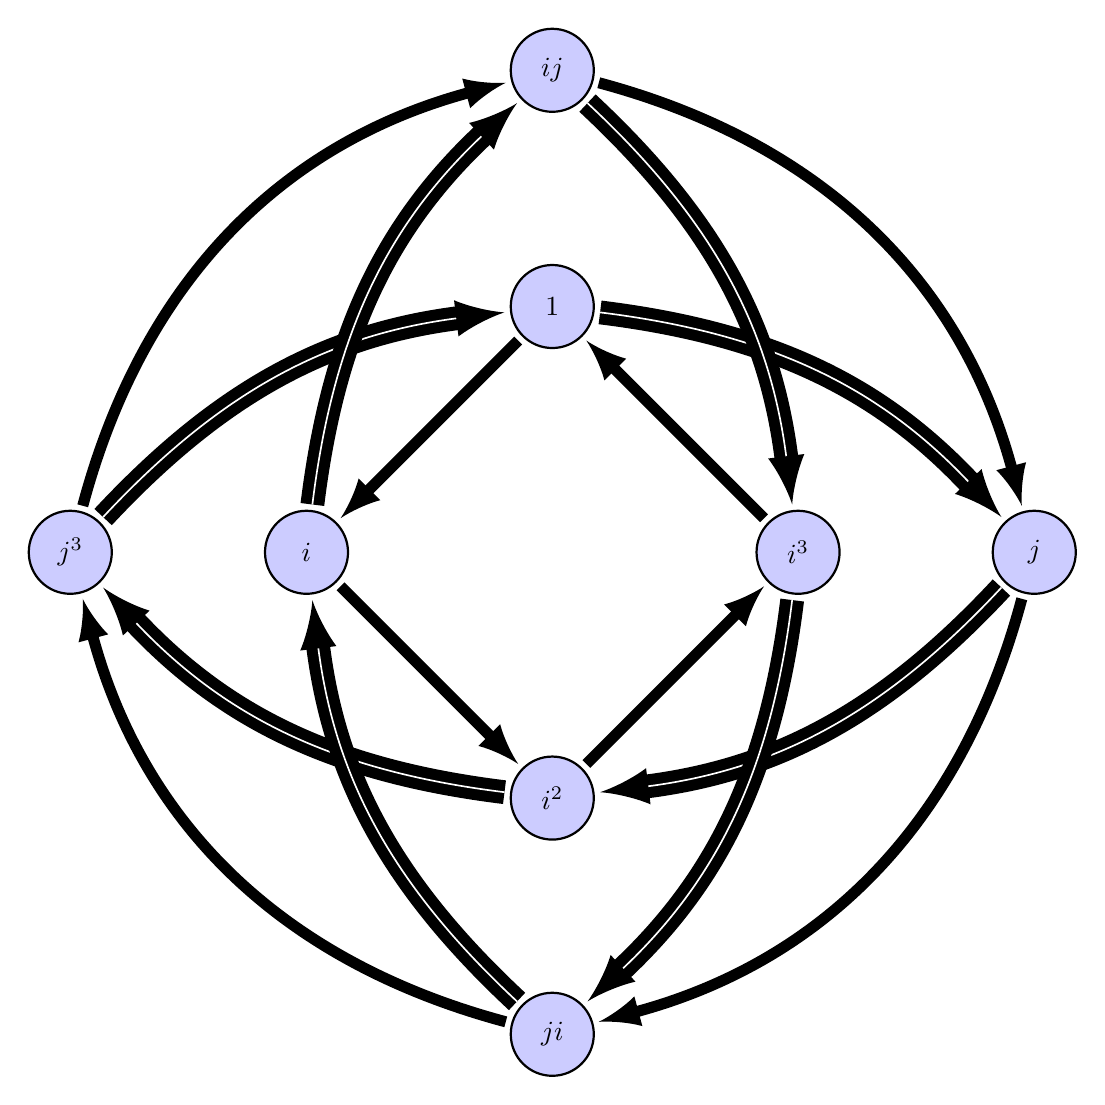
\begin{tikzpicture}[->,>=latex,shorten >=1pt,auto,node distance=3cm,
  thick,main node/.style={circle,fill=blue!20,draw}]

  \node[main node,minimum size=30pt] (ij) {\begin{math}ij\end{math}};
  \node[main node,minimum size=30pt] (1) [below of=ij] {\begin{math}1\end{math}};
  \node[main node,minimum size=30pt,yshift=-1cm,xshift=-1cm] (i) [below left of=1] {\begin{math}i\end{math}};
  \node[main node,minimum size=30pt] (j3) [left of=i] {\begin{math}j^3\end{math}};
  \node[main node,minimum size=30pt,xshift=1cm,yshift=-1cm] (i2) [below right of=i] {\begin{math}i^2\end{math}};
  \node[main node,minimum size=30pt] (ji) [below of=i2] {\begin{math}ji\end{math}};
  \node[main node,minimum size=30pt,xshift=1cm,yshift=1cm] (i3) [above right of=i2] {\begin{math}i^3\end{math}};
  \node[main node,minimum size=30pt] (j) [right of=i3] {\begin{math}j\end{math}};

  \draw[line width=4pt,shorten <=2pt,shorten >=2pt]
    % clockwise, outer
    (j3) edge [bend left] node[right] {} (ij)
    (ij) edge [bend left] node[right] {} (j)
    (j) edge [bend left] node[right] {} (ji)
    (ji) edge [bend left] node[right] {} (j3)
    % counter-clockwise, inner
    (1) edge node[right] {} (i)
    (i) edge node[right] {} (i2)
    (i2) edge node[right] {} (i3)
    (i3) edge node[right] {} (1)
    % bands
    (j3) edge [double,bend left=20] node[right] {} (1)
    (1) edge [double,bend left=20] node[right] {} (j)
    (j) edge [double,bend left=20] node[right] {} (i2)
    (i2) edge [double,bend left=20] node[right] {} (j3)
    (ij) edge [double,bend left=20] node[right] {} (i3)
    (i3) edge [double,bend left=20] node[right] {} (ji)
    (ji) edge [double,bend left=20] node[right] {} (i)
    (i) edge [double,bend left=20] node[right] {} (ij);

\end{tikzpicture}
\end{document}
